Earthquakes are an unpredictable phenomena, which damaging capabilities can be catastrophic. Given the scarse natural resources, its correct allocation is vital to mitigate the damage in the aftermath. Technology makes the labours of logistics and rescue a lot easier. This chapter explores the motivation, history, objective and scope of the present work.\\


\section{Motivation}


Massive collaboration proved to be a fundamental resource to face the aftermath caused by the earthquake of September 19, 2017 in Mexico City. The use of social networks allowed communication between rescue, logistics and civil society. Lessons were learned about the scope and limitations of this association.\\

However, what happens when the conditions and technological infrastructure of large cities do not exist? This work explores other possibilities in which current technologies can help us when the situation in which the natural disaster occurs is different. Focusing on the study of images captured by drones during the days after the earthquake of September 7, 2017 in towns of the state of Oaxaca, an analysis framework that allows to detect damaged areas in an automated way is proposed.\\

In order to do this, techniques are applied that allow the use of models that have been previously trained in gigantic infrastructures, adjusting them to our particular problem. This reduces the amount of resources needed, in both time and infrastructure, to obtain results with high accuracy. In the future, this will allow allocating efforts in a more agile and efficient manner.\\

\section{History}

Given to the particular geographical conditions, Mexico is very prone to seismic activity. The Cocos and the Rivera plates subduct below the North American plate, and the Pacific plate separates from the North American plate along the Baja California Gulf \cite{AG3315}.\\

According to historical research there have been registry of these natural disasters since the Pre-Columbian age. The level of material damage, and the death toll has incresing ever since as the popululation and the cities grew. In figure \cite{fig:codice} we can see a pictogram that acording to \cite{sismosmexico} means "in the year 11 rabbit the earth trembled during the night".\\


\begin{figure}[h]
  \begin{center}
    \subfigure{\label{fig:codice}\fbox{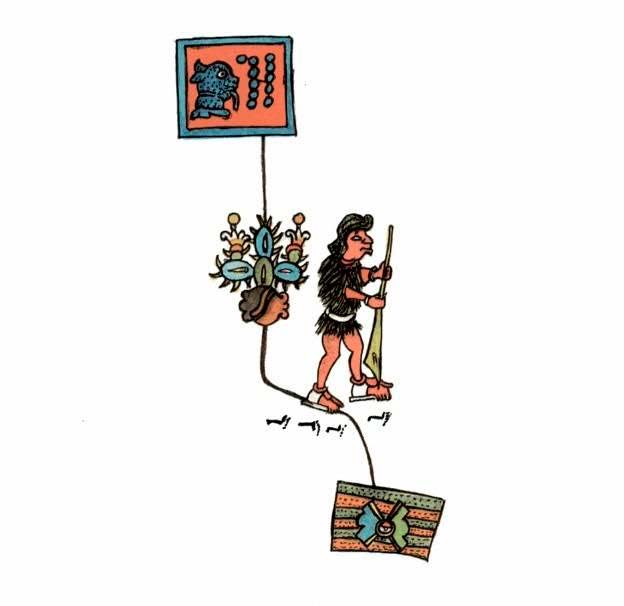
\includegraphics[width=1\textwidth]{images/codice.jpg}}}
  \end{center}
\end{figure}

The use of cartography to place the damage information also is useful not only to allocate resources in the aftermath of the disaster but also serves as historical evidence. In figure \cite{fig:quake1800} taken from \cite{AG3316} we can see the building that where damaged during an earthquake known as the *San Juan de Dios* earthquake \footnote{Back then the earthquakes where name acordingly to the day in which they happened.} that dates back to March 8, 1800, years before the Independence, during a age of economic and social prosperity.\\

Acoridng to historical records an important earthquake ocurred in the year 1787, causing a huge tsunami that afected the coasts of Oaxaca along 450 kilometers. Paradoxically, this catastrophic event didn't produced as much damage as recent ones due to the lack of stablished cities in the state back then.

Years 1845 and 1858 also had mayor earthquake events that destroyed infraestructure in Mexico city. We can find mapping of the damaged buldings in \cite{AG3316}.

The fall of the iconic Angel of Independence was the result of an earthquake on July 28, 1957 in an event that leave dozens of deaths.

Nevertheless the real breaking point in the Mexican seismological history came on September 19, 1985. That morning, an 8.1 magnitude earthquake stroke the city collapsing many buildings and leaving a death toll measured by thousands. Next day, the aftershock collapsed even more buildings that had been damaged the day before. The destruction and caos that the earthquake provoked still lingers in the memory of the people that witnessed such a terrifying event.

The way people reacted after September 19 2017 was largely because they grew up in an ambient of constant fear to the quakes. 

Two major earthquakes took place during the month of September 2017. While the second one devastated Mexico City, attracting help from all over the world, the first one was less known even though it was the earthquake with the greatest magnitude that has hit the country in the last century. Both where catastrofic for the state of Oaxaca. The locality of Juchitan de Zaragoza was one of the most affected, buildings collapsed, and several people died.

\begin{figure}[h]
  \begin{center}
    \subfigure{\label{fig:quake1800}\fbox{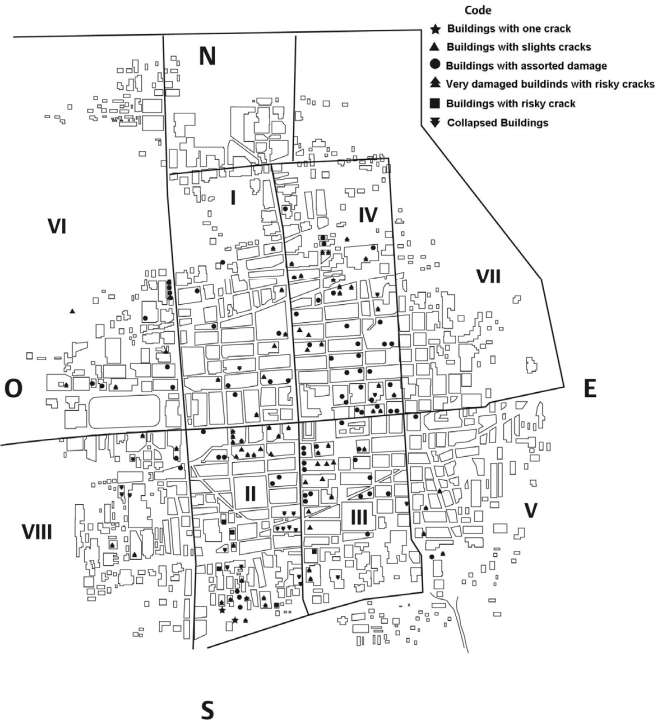
\includegraphics[width=1\textwidth]{images/quake1800.png}}}
  \end{center}
\end{figure}


\section{Objective}

It is not coincidental that our brief historical summary focused mainly in Mexico City. Historically, poorer states in Mexico have been constanly overlooked. The lack of infraestructure and the distance from large cities make it harder to reach certain towns with resources and aid. We want to explore the use of new technologies to focus our efforts and use them better. 

The National Center for Prevention of Disasters (CENAPRED) provided us with imagery taken on the days after the Chiapas earthquake took place. They flew drones over the towns of Juchitan de Zaragoza, Santa Maria Xadani and Union Hidalgo. We propose to use those images to train a model that lets us geolocate collapsed buildings and create a map with them. In the case of another catastrophic event of similar nature, drones can be sent to fly over the affected area and the map can be used to narrow dramatically the places which human assesment teams must visit. This would reduce the amount of resources and time needed to correctly asses the damage in the earthquake aftemath.

In Mexic, CENAPRED is in charge of channeling financial resources in the case of a natural disaster. 

We want to explore the use of Convolutional Neural Networks (CNNs) in this context. We believe that this field is very promising for disaster assesment, and will bloom in the comming years. 

\section{Scope}

We don't pretend to provide a perfect mapping of every single collapsed building. We understand the inherent limitations of automatic methods, but we beilieve that we can achieve greater things working together with this new tools. Machine learning methods are not a panacea by no means, but a useful device that can help us reach places we could just imagine before.

It is important to keep in mind that this is only the beginning and that there is huge room for improvement. The literature review in which we will dive deeper in the next chapter sugest ways of improving the results that we got, but its implementation is out of scope of this work.

It would be far too ambitious to cover every topic that is involved in the process of the classification using CNNs. We want to explain how do the networks work to a certain extent, but it is not in the scope of this work to untangle every single detail. In the same fashion, the field of Remote Sensing is far too big to be explored in this work. We assume a certain degree of knowledge in related topics and we expose some mathematical details in the appendix.\\

As we already mentioned, the field of Computer Vision is in its climax. Reviewing every single article that has been writen would be a daunting task. We offer a brief literature review that gives some context about the state-of-the art and we hope to build upon ideas and efforts done by a miryad of people. We aimed to built a system capable of procesing imagery and that could be deployed into a cluster for efficient computation.\\
